Vision is one of the most important senses for animals; humans use it extensively for all kinds of tasks. Hunting, assessing danger, reading, driving, drawing, predicting rain from grey clouds, etc., these are all tasks that involve \emph{seeing}. 

There is a vast collection of knowledge about the components of vision, though a unified theory of vision (or the answer to \emph{How do we see?}) has not yet been achieved.

Vision starts at the eye, which transforms electromagnetic radiation that assembles an image, into voltage pulses that our brain may interpret. This encoded images are sent to the posterior region of the brain through the optic nerves. The cortex then performs many computations that result in our ability to see.

\section{The eye and the retina}
\label{sec:vision:eye}
Our everyday experience might lead us to believe that the eyes are sensory organs developed completely separate from the brain but, in fact, the retina is an extension of the brain that performs spatio-temporal compression of a continuous flow of ``images'' of the world~\cite{eye-brain-vision-hubel1995}.

The eye is composed of many parts that resemble a mechanical camera (Figure~\ref{fig:vision:eye}). The cornea is a transparent film that protects the frontal part of the eye and encloses the eye. The lens is in charge of focusing light rays into the retina, which acts as a complex sensor that will be described further in the following paragraphs. The pupil and the iris act as a camera's aperture mechanism, the amount of light input is regulated by broadening or reducing the diameter of the pupil. 

\begin{figure}[htb]
  \begin{center}
    \includegraphics[width=0.5\textwidth]{simple-eye-anatomy}
    \caption{Simplified anatomy of the eye~\cite{webvision-images}.}
    \label{fig:vision:eye}
  \end{center}
\end{figure}

The retina is organized in layers of cell bodies or nerves,  Figure~\ref{fig:vision:simple-retina} shows a simplified version of the retina's anatomy~\cite{webvision-simple-retina}. Light enters the eye and has to travel all the way to the deepest part of the retina (right of Fig.~\ref{fig:vision:simple-retina}) to be sensed by the photoreceptors. 

\begin{figure}[h]
  \begin{center}
    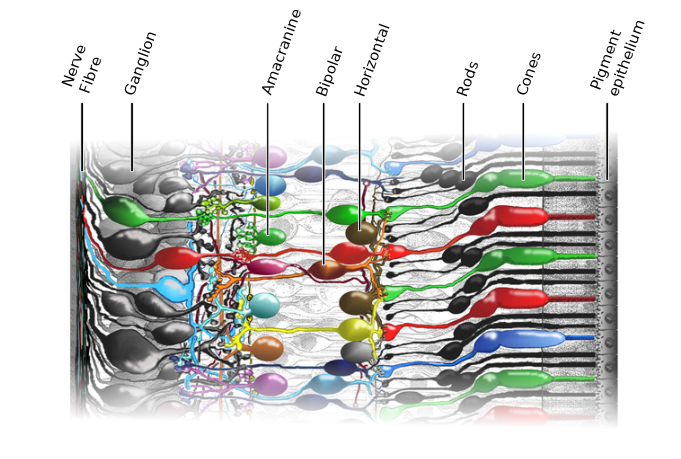
\includegraphics[width=0.7\textwidth]{retina-simple}
    \caption{Simple anatomy of the retina, adapted from~\cite{webvision-images}.}
    \label{fig:vision:simple-retina}
  \end{center}
\end{figure}

Photoreceptors transform light into an electrical signal. There are two primary types of photoreceptor cells within the retina: Colour is perceived by special type of receptors \emph{cones} and, contrast is perceived by \emph{rods}. Many mammals have retinas with more rods than cones, but primates' retinas are split in two separate zones. Most of the photosensitive area has more rods than cones but in a tiny region called the \emph{foveal pit}, there are almost no rods -- it's densely packed with cones. It is used for high-resolution vision and is virtually useless when there is not enough light~\cite{eye-brain-vision-hubel1995}.

The precise function of the other cell types is still a matter of debate and research. What is known is that \textbf{horizontal} cells  spatially average the input from photoreceptors and transmit to bipolar, which in turn output to ganglion cells. Horizontal cells also send a feedback signal to the photoreceptors, perhaps to adapt to different light conditions. \textbf{Bipolar} cells, as their name suggests, have outputs both to ganglion cells and photoreceptors. These first cell types (photoreceptors, horizontal and bipolar cells) use analog signals and feed ganglion cells which have a \emph{centre-surround} behaviour~\cite{eye-brain-vision-hubel1995,thompson2000brain}. Figure~\ref{fig:vision:centre-surround} illustrates the reaction of the two variants of centre-surround cells to different inputs.

\begin{figure}[h]
  \begin{center}
    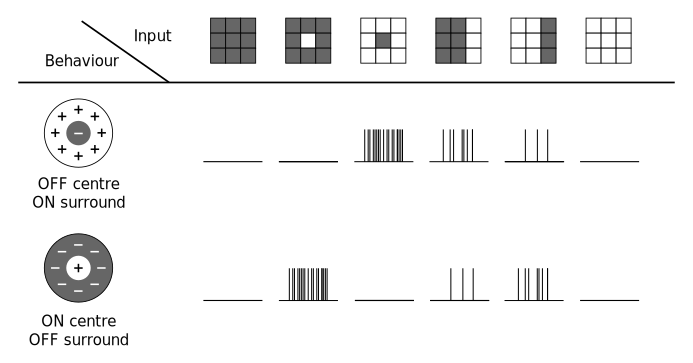
\includegraphics[width=0.7\textwidth]{centre-surround}
    \caption{Responses of centre-surround cells to different types of input.}
    \label{fig:vision:centre-surround}
  \end{center}
\end{figure}


\textbf{Ganglion} cells take input from bipolar cells, some form the surround (signal adapted by horizontal cells) and others the centre (pure signal from the photoreceptors). The centre-surround behaviour has been modelled by many authors using \emph{Laplacian of Gaussians} or \emph{Difference of Gaussians} ~\cite{thorpe-rate-coding-theory,virtual-retina,webvision-midget}. The output of ganglion cells are action potentials which are transmitted by the ganglion's axons, into the Lateral Geniculate Nucleus (LGN).

It's likely that most of the information sensed by the retina is redundant, this would keep the eyes working adequately even if some cells cease to function. To avoid saturation of nerve fibres and over-representation, lateral inhibition might play a big role~\cite{basab-model,thorpe-rate-coding-theory,field-sensory-coding}. The use of centre-surround responses in the retina is believed to help the eye overcome variations in lightning conditions, because the response comes from the contrast comparison between photoreceptors.

%After the light rays have been encoded into a neural representation, the optic nerve transfers the information to the Lateral Geniculate Nucleus (LGN) and from there to the visual portion of the cortex. A huge difference between a camera and the eye is that the latter maintains a continuous stream of information unlike the frame-based nature of cameras.

\section{The visual cortex}
\label{sec:vision:cortex}
At the end of last section, we stated that information from ganglion cells extend to the Lateral Geniculate Nucleus (LGN), where information is relayed and organized so that the cortex can interpret it. Organization makes left visual field sent to right hemisphere, right field to left hemisphere (Figure~\ref{fig:vision:optic-chiasm}).

\begin{figure}
  \begin{center}
    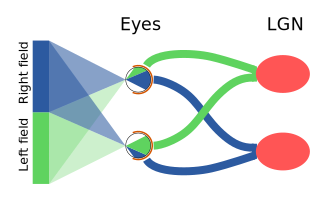
\includegraphics[width=0.7\textwidth]{visual-fields-lgn}
    \caption{Visual field mapping in LGN.}
    \label{fig:vision:optic-chiasm}
  \end{center}
\end{figure}

The portion of the cortex that is involved with visual processing has been estimated to about 30\%.

It has been studied and areas have been labelled due to their function.

V1, 
The primary visual cortex (V1) is the best-studied visual area in the brain.
correspondence between a given location in V1 and in the subjective visual field is very precise
 fovea in the retina, a large portion of V1 is mapped to the small, central portion of visual field
neuronal responses can discriminate small changes in visual orientations, spatial frequencies and colors. 
described as edge detection. 

V2
connections from v1 sends to v3,v4,v5 back to b1
more complex shapes than v1

V3
controversy still exists regarding the exact extent of area V3,
 it may contain a complete visual representation
  may play a role in the processing of global motion
  
V4
strong feedforward input from V2 and sending strong connections to the PIT
receives direct inputs from V1, especially for central space
it has weaker connections to V5 and dorsal prelunate gyrus (DP).
show strong attentional modulation
orientation, spatial frequency, and color.
tuned for object features of intermediate complexity, like simple geometric shapes
V4 is not tuned for complex objects such as faces, as areas in the inferotemporal cortex are

V5
Visual area V5, also known as visual area MT (middle temporal), is a region of extrastriate visual cortex that is thought to play a major role in the perception of motion, the integration of local motion signals into global percepts, and the guidance of some eye movements.


V6
sharp selectivity for the orientation of visual contours, and preference for long, uninterrupted lines covering large parts of the visual field
strongly responsive to low spatial frequency components of an image, and respond poorly to the motion of textured pattern


\section{Conclusions}
\label{sec:vision:conclusions}
\section{Conclusion}
\section{Further work}
\section{Plans for second and third year}

%\section{Eyes for computers}
%Traditionally cameras have been used as they work similar to the first stage of the eye.

Recently dynamic vision sensor

They work in a way that more resembles the retina, event based

Still need development, resolution is low, they do not perform multiple-scale
convolution, expensive

A mix of both can be a great tool for researchers and commercial applications see Chp \ref{chp:img2spk}
%\label{sec:vision:cameras}
